\documentclass[12pt,a4paper]{article}
\usepackage{adjustbox} % in preamble

\usepackage[utf8]{inputenc}
\usepackage[latvian]{babel}
\usepackage{caption}
\usepackage{hyperref}

% Make captions "1. attēls."
\DeclareCaptionLabelFormat{numberfirst}{\arabic{figure}. attēls}
\captionsetup[figure]{labelformat=numberfirst,labelsep=period}

% Command for referencing: "1. attēls"
\newcommand{\figref}[1]{\ref{#1} attēls}


\pagenumbering{arabic} % Sets page numbering to arabic (1, 2, 3, ...)
\setcounter{page}{1} % Specifies the starting page number

\usepackage{tabularx} % in your preamble
\usepackage{amsmath, amssymb}
\usepackage{graphicx}
\usepackage{geometry}
\usepackage{subcaption}
\usepackage{float}
\usepackage{array}
\usepackage{booktabs}
\usepackage{enumitem}
\usepackage{fancyhdr}
\usepackage{xcolor}
\usepackage{framed}
\usepackage{titlesec}
\usepackage{breakurl}   % optional if hyperref is used with breaklinks

% Example 1: Bold, larger font, with some vertical spacing
\titleformat{\section}
  {\normalfont\Large\bfseries} % format: font + weight
  {\thesection}                % label (number)
  {0.3em}                         % space between number and title
  {}                            % code before title text

\geometry{
    left=2cm,
    right=2cm,
    top=2.5cm,
    bottom=2.5cm
}

\pagestyle{plain}
\fancyhf{}
\rhead{Olbaltumvielas}

% Custom colors and environments
\definecolor{taskbg}{rgb}{0.95,0.95,0.95}

% Custom environment for tasks
\newenvironment{taskbox}
{\begin{framed}\begin{minipage}{\textwidth}}
{\end{minipage}\end{framed}}

\title{\textbf{Tests par augu pigmentiem}}
\author{}
\date{}

\begin{document}

\maketitle


\noindent \textbf{1. jautājums.} Kuri ir primārie augu fotosintēzes pigmenti? 
\begin{enumerate}[label=\Alph*.]
    \item hlorofili
    \item karotīni
    \item betalaīni
    \item antocianīni
\end{enumerate}
\noindent \textbf{2. jautājums.} Kuri apgalvojumi par hlorofilu nav patiesi?

\begin{enumerate}[label=\Alph*.]
    \item Hlorofils atstaro zaļo gaismu.
    \item Hlorofils laiž cauri zaļo gaismu.
    \item Hlorofils pilnībā absorbē zaļo gaismu.
    \item Hlorofils vispār neabsorbē zaļo gaismu.
\end{enumerate}

\noindent \textbf{3. jautājums.} Kura absorbcijas līkne \ref{fig:hlorofili} attēlā pieder hlorofilam a un kura — hlorofilam b, ja hlorofils a ir zilāks par b?
\begin{figure}[H]
    \centering
    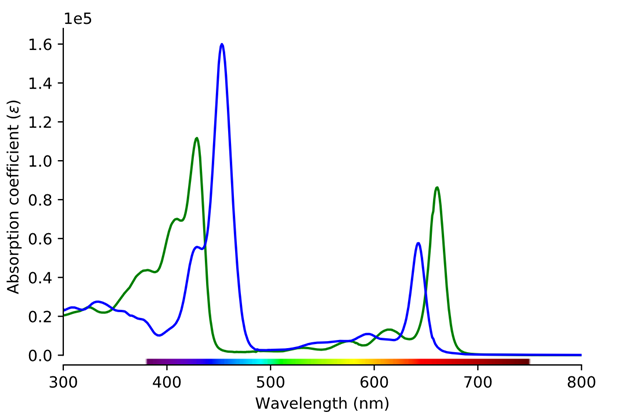
\includegraphics[width=0.5\textwidth]{atteli/hlorofili.png}
    \caption{Hlorofilu absorbcijas līknes.}
    \label{fig:hlorofili}
\end{figure}

\newpage

\noindent \textbf{4. jautājums.} Kura nav karotenoīdu funkcija? 

\begin{enumerate}[label=\Alph*.]
    \item aizsardzība pret lieko fotonu enerģiju un brīvajiem radikāļiem
    \item sēklu izplatītāju pievilināšana
    \item sekundārā gaismas absorbcija
    \item kamuflāžas nodrošināšana
\end{enumerate}

\begin{figure}[h]
    \centering
    \begin{minipage}[c]{0.55\textwidth} % Left side: question
        \textbf{5. jautājums.}  Kādi pēc to ķīmiskās uzbūves ir karotenoīdi (\figref{fig:karotenoidi})?

        \begin{enumerate}[label=\Alph*.]
            \item hidrofobi
            \item hidrofili
            \item amfifili
        \end{enumerate}
    \end{minipage}%
    \hfill
    \begin{minipage}[c]{0.40\textwidth} % Right side: image
        \centering
        \adjustbox{valign=c}{%
            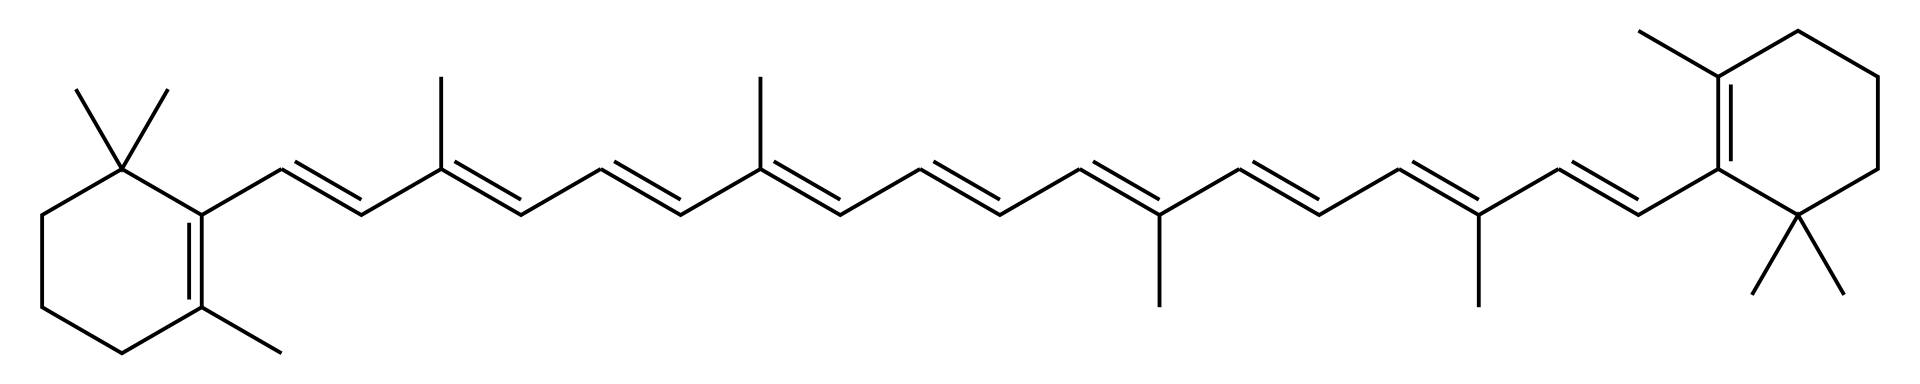
\includegraphics[width=0.7\textwidth]{atteli/karotins.png}}
        \caption{~}
        \label{fig:karotenoidi}
    \end{minipage}
\end{figure}

\noindent \textbf{6. jautājums.} Kuri no dotajiem nav karotenoīdi?

\begin{enumerate}[label=\Alph*.]
    \item  karotīni
    \item ksantofili
    \item antocianīni
\end{enumerate}

\noindent \textbf{7. jautājums.} Ksantofili ir dzelteni karotenoīdi ar hidroksilgrupām (—OH) un karotīni ir oranži un sarkani bez hidroksilgrupām. Kāda veida karotenoīds ir luteīns (ksantofils vai karotīns)? 

\begin{figure}[H]
    \centering
    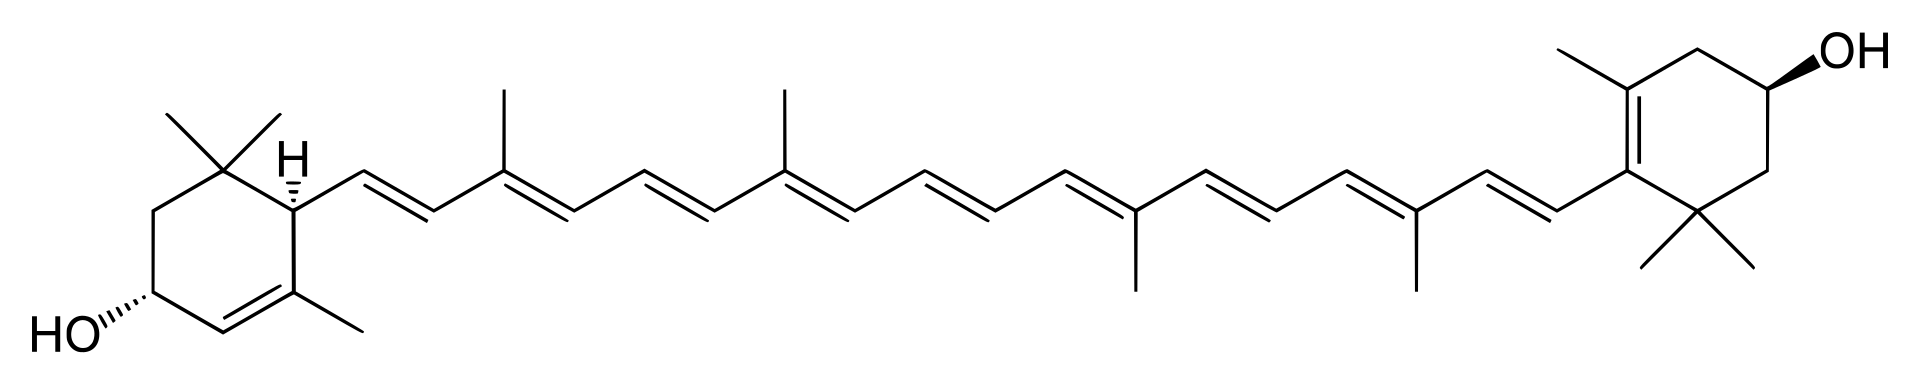
\includegraphics[width=0.5\textwidth]{atteli/lutein.png}
    \caption{Luteīns.}
    \label{fig:luteins}
\end{figure}

\noindent \textbf{8. jautājums.} Kurš ir svarīgāks redzei — luteīns vai $\beta$ karotīns? 


\noindent \textbf{9. jautājums.} Sarindo antocianīnu krāsas sākot no zema līdz augstam pH!

\begin{enumerate}[label=\Alph*.]
    \item zili-bezkrāsaini-zaļi
    \item zili-bezkrāsaini-sarkani
    \item sarkani-bezkrāsaini-zili 

\end{enumerate}

\noindent \textbf{10. jautājums.}Vai hortenziju krāsa \ref{fig:hortenzijas} attēlā atbilst antocianīnu krāsojumam iepriešējā jautājumā?

\begin{figure}[H]
    \centering
    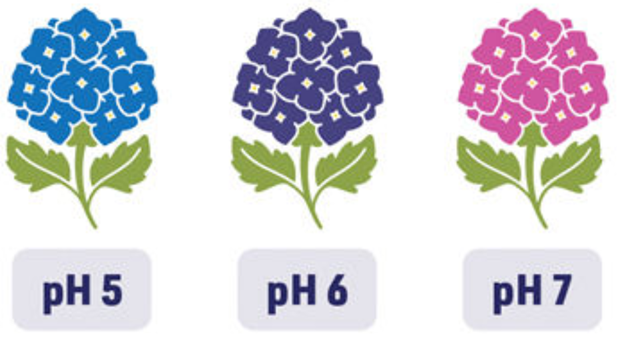
\includegraphics[width=0.5\textwidth]{atteli/hydrangea.png}
    \caption{~}
    \label{fig:hortenzijas}
\end{figure}



\section*{Atsauces}
\sloppy
\begin{enumerate}[leftmargin=*]
    \item Des\_Callaghan, CC BY-SA 4.0, via Wikimedia Commons
    \item Serge Helfrich, CC BY-SA 4.0, via Wikimedia Commons
    \item NEUROtiker, Public domain, via Wikimedia Commons
    \item By Yikrazuul - Own work, Public Domain, Link
    \item Lei Zhao, Yaqi Liu, Liang Zhao, Yong Wang, \textit{Anthocyanin-based pH-sensitive smart packaging films for monitoring food freshness}, Journal of Agriculture and Food Research, 2022.
    \item C\&EN, A. B. S. T. (2024, May 3). \textit{Periodic Graphics: The chemistry of hydrangea color changes}. Chemical \& Engineering News. \url{https://cen.acs.org/environment/Periodic-Graphics-chemistry-hydrangea-color/102/i13?sc=240428_sc_eng_fb_cen}

\end{enumerate}


\newpage
\section*{Atbildes}

\begin{enumerate}
\item A.
\item C un D. No visām krāsām hlorofili vismazāk absorbē zaļo, tāpēc tos tādus redzam, taču nav tā, ka tie vispār to neabsorbē.
\item Hlorofilam a pieder zaļā līkne, jo tas absorbē mazāk zilas gaismas.
\item D. Spilgti dzeltenās, oranžās, sarkanās karotīnu krāsas pievilina dzīvniekus.
\item A. Attēlā redzams, ka tie sastāv tikai no ogļūdeņražu ķēdes un cikliem.
\item C. Ksantofili ir dzelteni karotenoīdi ar hidroksilgrupām (—OH) un karotīni ir oranži un sarkani bez hidroksilgrupām.
\item Ksantofils, jo tam ir hidroksilgrupas. Luteīns ir sarkanais pigments tomātos.
\item Luteīns un zeaksantīns ir makulas pigmenti, kuri aizsargā acu fotoreceptorus no zilās gaismas (\figref{fig:makula}).
\item C. Lai izprastu turpmāko, izlasi materiālu par ķīmiskajām saitēm. Tagad aplūko \ref{fig:antocianini} attēlu. Zemā pH antocianīni ir protonēti. —OH grupas spēj labi ziedot elektronus, tāpēc delokalizē elektronu blīvumu (jeb elektroni tiek dalīti pa visu molekulu, nevis atsevišķām saitēm). Šādi $\pi$ sistēma tiek stabilizēta un absorbēta tiek augstākas enerģijas jeb zemāka viļņa garuma gaisma, piemēram, zilā. Tā kā tiek absorbēta zila, zemā pH redzamā krāsa ir sarkana. Karbonilgrupas C=O neziedo elektronus, tāpēc $\pi$ sistēma netiek stabilizēta un nevajag tik daudz enerģijas gaismas absorbcijai.
\item Nē, hortenzijas ir zilas zemā pH, taču bioloģijas brīnumu kārtā hortenziju krāsu nodrošina antocianīns — delfinidīns. Taču šajā gadījumā tas nav tikai pH un antocianīna ķīmiskā struktūra, kas nosaka krāsu, bet arī alumīnija joni. Tie zemē atbrīvojas zemā pH, tādējādi kopā ar delfinidīnu krāsojot hortenzijas zilas zemā pH.

\end{enumerate}

\begin{figure}[H]
    \centering
    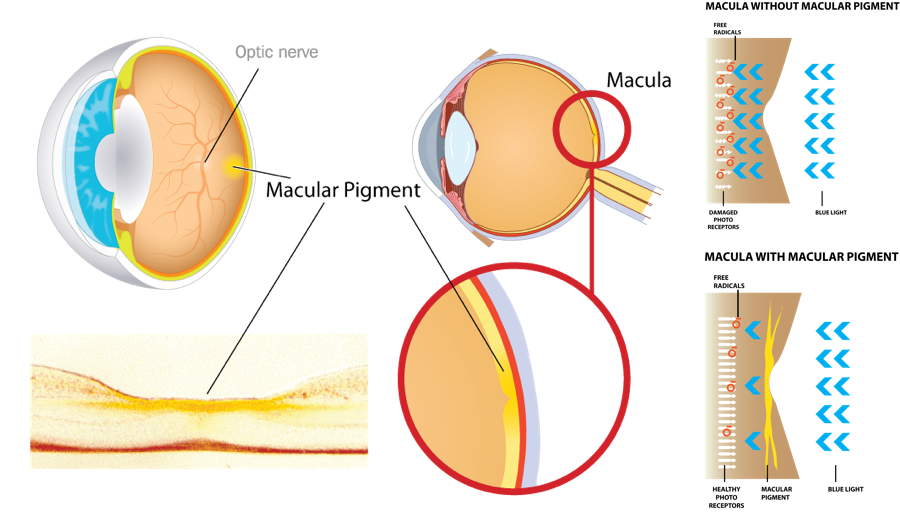
\includegraphics[width=0.5\textwidth]{atteli/makula.png}
    \caption{Makulas uzbūve.}
    \label{fig:makula}
\end{figure}

\begin{figure}[H]
    \centering
    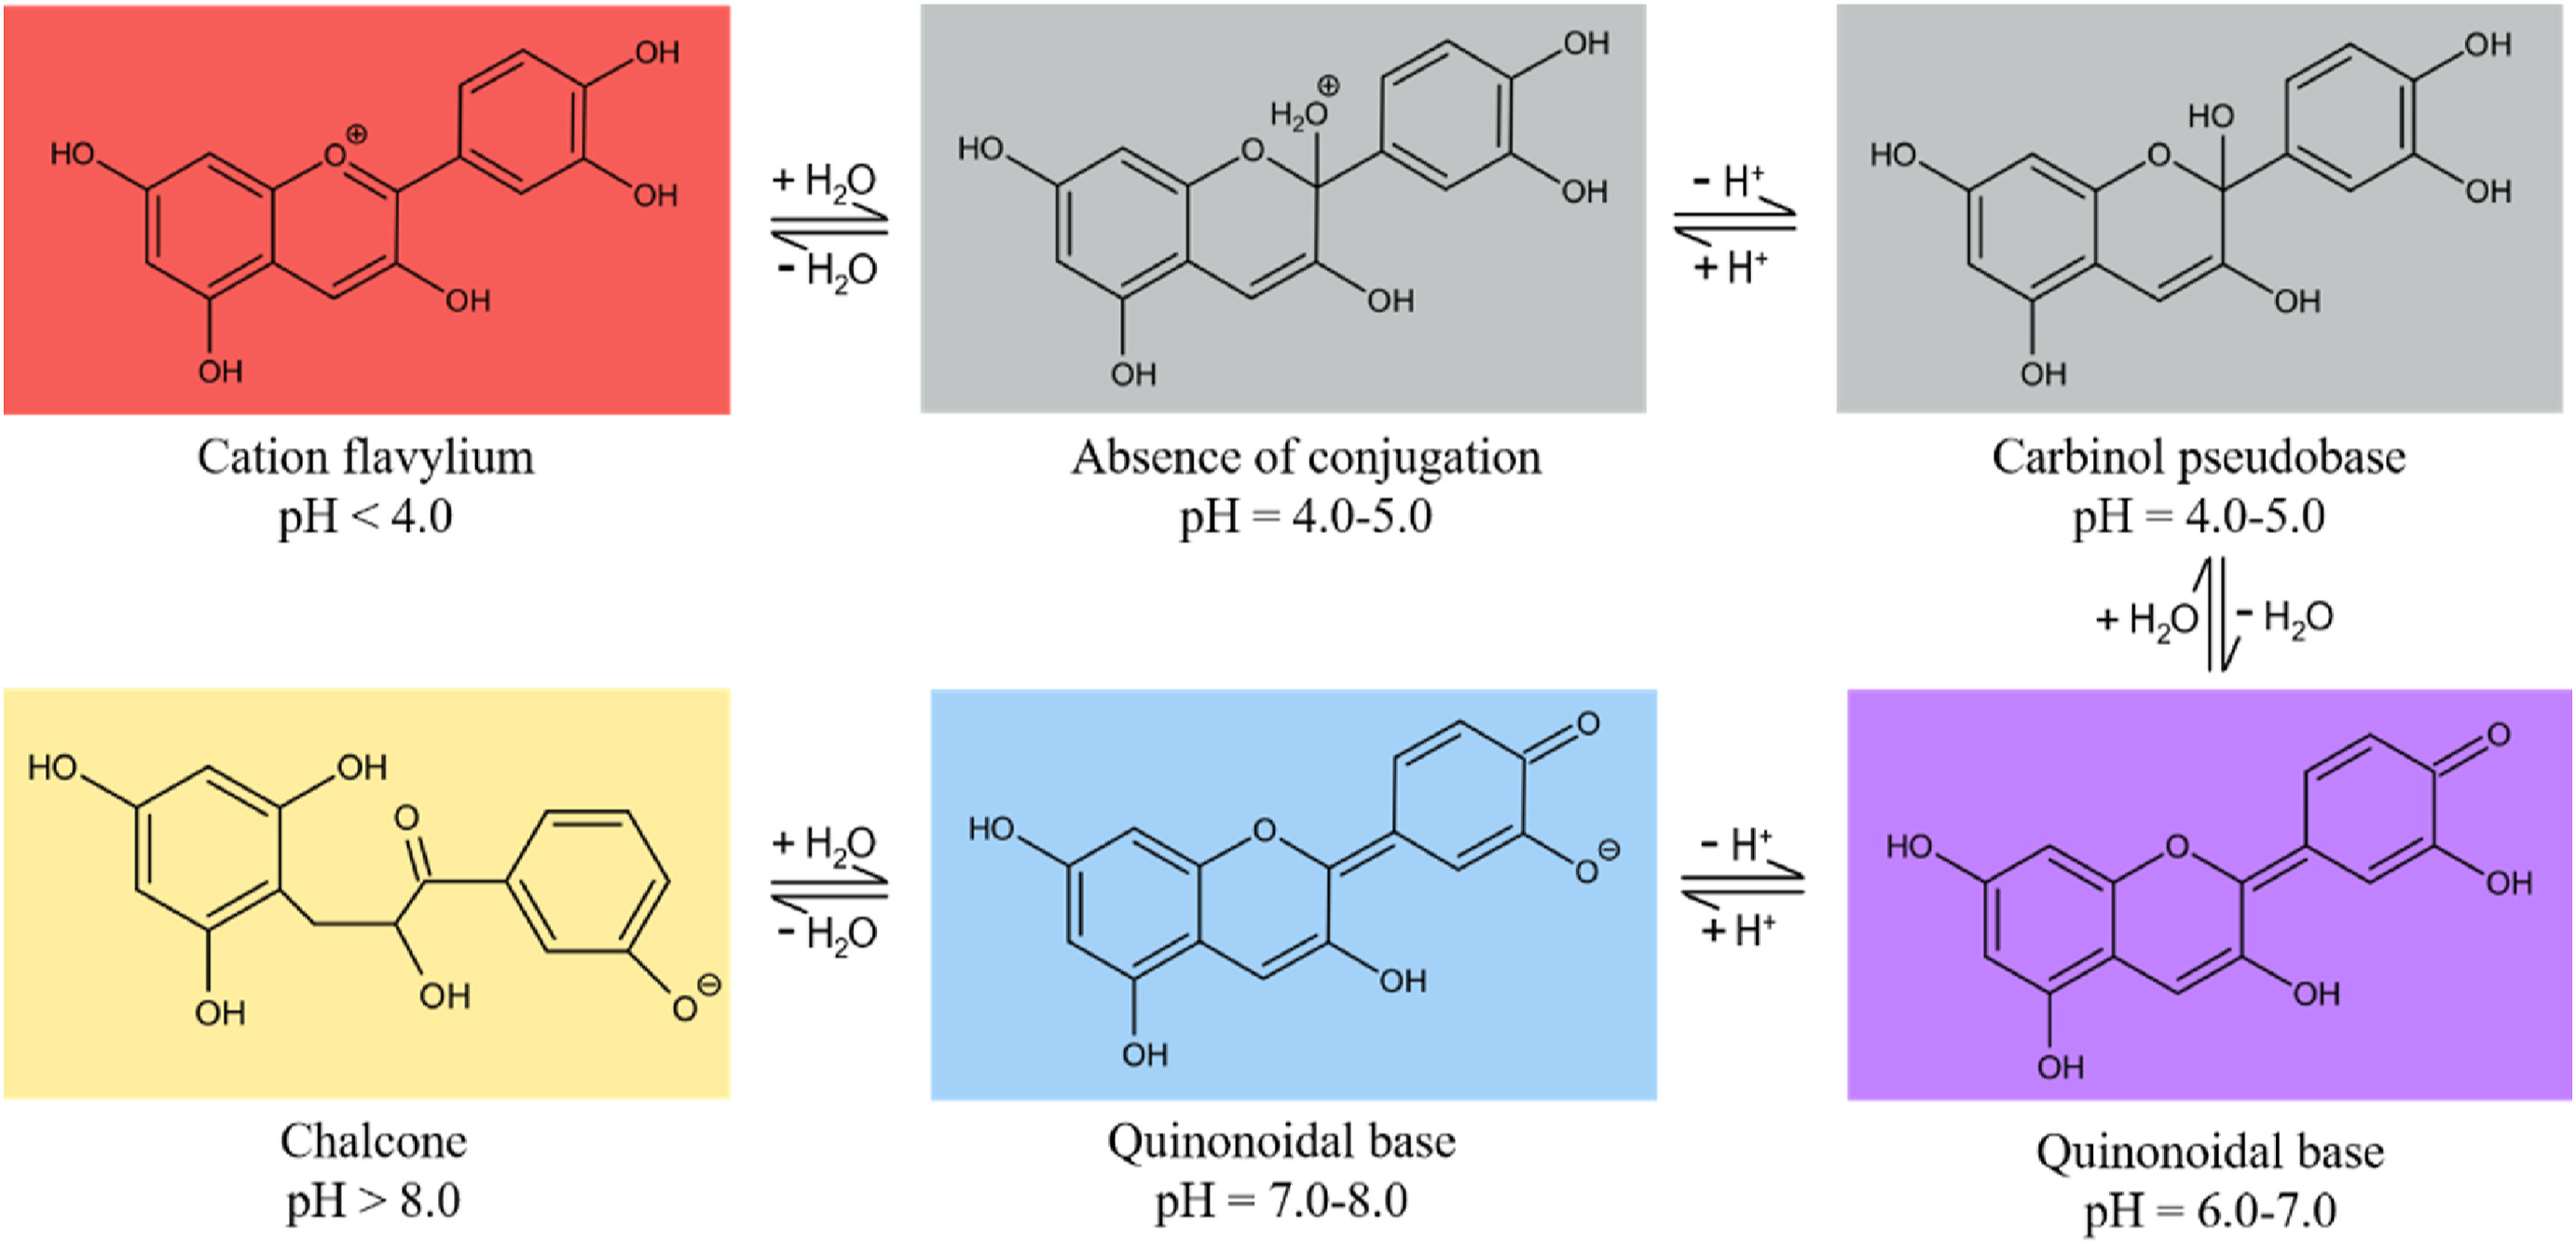
\includegraphics[width=0.5\textwidth]{atteli/antocianini.jpg}
    \caption{Antocianīni.}
    \label{fig:antocianini}
\end{figure}

\end{document}